% ===========================================================================
% Title:
% ---------------------------------------------------------------------------
% to create Type I fonts type "dvips -P cmz -t letter <filename>"
% ===========================================================================
\documentclass[11pt]{article}       %--- LATEX 2e base
\usepackage{latexsym}               %--- LATEX 2e base
\usepackage[table]{xcolor}
\usepackage{tikz}
\usetikzlibrary{shapes}
\usepackage{forest}
\usepackage{adjustbox}
\usepackage{amsmath}
\usepackage{pgfplots}
%---------------- Wide format -----------------------------------------------
\textwidth=6in \textheight=9in \oddsidemargin=0.25in
\evensidemargin=0.25in \topmargin=-0.5in
%---------------- Custom Colors -----------------------------------------------
\definecolor{darkGreen}{HTML}{186A3B}
\definecolor{orange}{HTML}{D35400}
%--------------- Def., Theorem, Proof, etc. ---------------------------------
\newtheorem{definition}{Definition}
\newtheorem{theorem}{Theorem}
\newtheorem{lemma}{Lemma}
\newtheorem{corollary}{Corollary}
\newtheorem{property}{Property}
\newtheorem{observation}{Observation}
\newtheorem{fact}{Fact}
\newenvironment{proof}           {\noindent{\bf Proof.} }%
                                 {\null\hfill$\Box$\par\medskip}
%--------------- Algorithm --------------------------------------------------
\usepackage[ruled, lined, vlined, linesnumbered]{algorithm2e}
%--------------- Figures ----------------------------------------------------
\usepackage{graphicx}

\newcommand{\includeFig}[3]      {\begin{figure}[htb] \begin{center}
                                 \includegraphics
                                 [width=4in,keepaspectratio] %comment this line to disable scaling
                                 {#2}\caption{\label{#1}#3} \end{center} \end{figure}}
                                 % usage: \includeFig{label}{file}{caption}


% ===========================================================================
\begin{document}
% ===========================================================================

% ############################################################################
% Title
% ############################################################################

\title{Top Down Specialization on Apache Spark\texttrademark}


% ############################################################################
% Author(s) (no blank lines !)
\author{
% ############################################################################
Macarious Abadeer\\
School of Computer Science\\
Carleton University\\
Ottawa, Canada K1S 5B6\\
{\em macariousabadeer@cmail.carleton.ca}
% ############################################################################
} % end-authors
% ############################################################################

\maketitle

% ############################################################################
% Abstract
% ############################################################################
\begin{abstract}
A very concise summary of the problem addressed and solution presented in this paper.
\end{abstract}


% ############################################################################
\section{Introduction} \label{intro}
% ############################################################################

Since the introduction of multi-core processors in 2004 by Intel\textsuperscript{\textregistered}, parallel computing evolved to exploit the advantages of multiple processing units that became the norm for personal computers. This evolution was also expanded and accelerated by the advancements in Cloud Computing that supported running compute-intensive applications over a network of clusters. Parallel computing enabled the development of solutions to different real world applications that were hindered by scalability limitations such as big data analytics, machine learning and artificial intelligence. One of the problems that parallel computing provided scaleable solutions for is data anonymization, especially for big data. 

In today's abundance of big data ranging from retail and banking transactions, health care, social media interactions and sensor data, a need was created for measures that protect people's most private and sensitive data. One of the most popular theories that were developed in this area was $k$-anonymity developed by Samarati and Sweeney in 1998 \cite{Samarati-P.:1998}. Sweeney argued that an individual in a dataset can be identified when the dataset is linked with other public datasets even if the original dataset did not contain identifying information such as name, date of birth and social insurance number. Sweeney was able to show that when linking voter registration cards and health care data, individuals can be identified with 87\% accuracy. Those potentially identifying attributes are called Quasi-Identifiers (QID). $k$-anonymity states that a dataset is called $k$-anonymous when for a given record, there exists at least \(k-1\) records in the same dataset with the same QID values.  Further modifications to $k$-anonymity were made to overcome its shortcomings such as introducing $\ell$-diversity \cite{Machanavajjhala:2007} and $t$-closeness \cite{Li-N.:2007}. $\ell$-diversity ensures that sensitive attributes, such as diagnosis in a health care dataset, need to have diverse values so that an adversary with foreknowledge of a given QID set cannot deduce their diagnosis. $t$-closeness ensures that the distribution of these diverse values is close to their distribution in the original dataset.

While these theories contributed immensely to the practices of data anonymization, $k$-anonymity was proven to be $\mathcal{NP}$-hard by Meyerson and Williams \cite{Meyerson:2004}. Further research used these models as a baseline to develop scalable parallel algorithms that can handle big data.

The paper is organized as follows: in Section~\ref{literature}, I will go over the different ideas that were proposed to optimize and scale $k$-anonymity. Section~\ref{solution} will detail an implemented proposed solution and Section~\ref{evaluation} presents the experimentation results of the algorithm and the paper finally concludes in Section~\ref{conclusion}.


% ############################################################################
\section{Literature Review} \label{literature}
% ############################################################################

There are three different masking types that are used to satisfy $k$-anonymity: interval, taxonomy tree and suppression \cite{Al-Zobbi-Mohammed:2018}. Suppression requires certain outlier tuples to be removed to satisfy $k$-anonymity \cite{Samarati-P.:1998}. Intervals and taxonomy trees are generalization techniques applied to numerical and categorical attributes respectively \cite{Samarati-P.:1998}. For example two records with birth year of 1971 and 1973 can be generalized to 1970-1975. For a taxonomy tree, a categorical attribute such as education level can have, for example, post-graduate as a parent node which can have PhD, Masters and Post Graduate Diploma as its child leaves so that records with these values can be generalized to the parent node. The majority of research papers on anonymization with respect to big data involved taxonomy trees thus this is where I focus my literature survey.

One of the techniques that researchers attempted to optimize was Bottom-Up Generalization (BUG) which involves traversing the taxonomy tree of attribute hierarchies from the bottom (most specific) upwards (most general) \cite{Ke-Wang:2004}. Wang suggested that the taxonomy tree would be provided by the data supplier or the data recipient \cite{Ke-Wang:2004}. As the tree is traversed, two metrics are calculated to ensure a high quality generalization: information loss and anonymity gain. An indexed approach to bottom-up generalization was proposed by Hoang \cite{Hoang:2012} where the taxonomy tree was generated automatically at runtime. Hoang's indexed approach could also handle numerical as well as categorical attributes. Indexed BUG starts with collecting statistical information about the dataset as well as partition it so that it can be used in the generalization step which was further broken down to four steps: calculate the best generalization score based on the least information loss, calculate $k$-anonymity for every partition, generate an indexed generalization map which maps every value to its generalized value, and the last step creates the anonymized dataset using this map. Hoang's experiments showed that the generalization time did not increase with the dataset size due to the use of indexed generalization map however performance was impacted by the distinct values count for each QID \cite{Hoang:2012}.

Parallel BUG was introduced to address the limitations of traditional and indexed BUG approaches. Pandilakshmi attempted to solve the limitations of indexing structures since they are centralized and hard to parallelize and cannot run on distributed systems such as the Cloud \cite{Pandilakshmi:2014}. Pandilakshmi introduced Bi-Level BUG algorithm where MapReduce framework was used to take advantage of job-level and task-level parallelization. Job-level parallelization was achieved by using multiple MapReduce jobs and task-level parallelization was achieved by using multiple mapper/reducer tasks for every MapReduce job so that they are executed in parallel on every partition. Data is partitioned according to a random number generated between 1 and $p$ where $p$ is the number of partitions. Pandilakshmi then runs MapReduce BUG driver (MRBUG) iteratively on the partitioned datasets and calculates generalization score (least information loss with the most anonymity gain) and stops until it finds the best generalization with the highest score that satisfies $k$-anonymity. Pandilakshmi experiments performed on varying datasets of up to 4GB showed that execution time was virtually capped at $\approx$33 minutes regardless of dataset size.

Another technique is Top-Down Specialization (TDS). TDS traverses the taxonomy tree from the top downwards where it starts with the most generalized values and specializes the value and stops when it violates $k$-anonymity \cite{Fung:2005}. Multiple solutions have been developed such as a scalable two-phase TDS introduced by \cite{Priyanka:2014} and \cite{Zhang:2014}. The first phase involves partitioning the original dataset to $p$ partitions using random sampling. A MapReduce TDS job runs in parallel on each partition. Each job specializes the data iteratively while calculating information gain and privacy loss metrics and creates an intermediate anonymized dataset. In the second phase the intermediate datasets are merged and further anonymized if necessary to satisfy $k$-anonymity. In \cite{Zhang:2014}, Zhang et al. adopted Hadoop\textsuperscript{\textregistered} and took advantage of distributed cache capability to pass the intermediate anonymized dataset to each mapper/reducer node. The experiments for this solution showed an overhead in the partitioning phase of the dataset.

A hybrid approach of BUG and TDS using MapReduce was introduced by \cite{Zhang:2013} where it was shown that when either TDS or BUG were used individually, they performed poorly for certain values of $k$. The hybrid approach applies TDS for large $k$ values and BUG for smaller ones. The notion of Workload Balancing Point was introduced which is defined as the point where the amount of computation required for TDS is the same as BUG. Once that point is identified, the hybrid approach chooses TDS for $k$ greater than the workload balancing point and chooses BUG when $k$ is smaller. The workload balancing point is estimated using the height of the taxonomy tree as a reference.

Al-Zobbi et al \cite{Al-Zobbi-Mohammed:2018} argued that finding the highest scoring generalization and specialization based on information gain and anonymity loss in BUG and TDS require high computational costs and impedes the ability to parallelize them. Al-Zobbi also argued that as the data grows in size, the high accuracy of these computations no longer make a statistical difference. Al-Zobbi proposed a multi-dimensional sensitivity-based algorithm on Apache Spark that uses a pre-determined QID attributes to anonymize as well as precalculated $k$ value using linear regression. The solution also takes into consideration the probability value of each QID. For example assuming that age can range between 1 and 100, the probability of finding a given age is 1\% which is much higher than a probability of finding a given job title assuming there are 200 different job titles. The solution prioritized the anonymization of higher probability attributes instead of calculating information gain and anonymity loss scores for every attribute. The solution also used a role-based access control equivalent system to set $k$ based on context. For example a health care dataset maybe given a lower $k$ (less anonymization) when shared with a doctor but a higher $k$ value when shared with an insurance risk analyst. The solution was implemented on Spark and aimed at minimizing the use of User Defined Functions (UDFs) since they run outside of the Spark JVM which is beyond the resource negotiator's control. Al-Zobbi recognized that this solution would sacrifice the analytical value of the dataset for the performance improvement gained by not calculating the best generalization options.

In a research paper by \cite{Shi:2015}, a survey was done on MapReduce vs. Spark for big data analytics. It concluded that Spark is better suited for problems that require accessing the same dataset multiple times such as the case with both TDS, BUG and their variants. The constant read and write by Hadoop to HDFS (Hadoop Distributed File System) is considered a significant overhead however Spark operates on datasets in memory and provides the capability of caching Resilient Distributed Datasets (RDDs) for faster access making it suitable for iterative algorithms. The experiments carried out by Shi et al in \cite{Shi:2015} found that Spark is 5 times faster than MapReduce for iterative algorithms regardless of data size.

Shi's findings in \cite{Shi:2015} are inline with other researchers that implemented anonymization algorithms on Spark such as \cite{Canbay:2017} and \cite{Sopaoglu:2017}. For example, \cite{Sopaoglu:2017} proposed a TDS implementation for Apache Spark that partitioned the dataset to $p$ partitions on $n$ Spark nodes where \(n=p\). The master node partitions the data and calculates the scores required by TDS such as information gain and privacy loss. The scores are sent to the driver node which performs aggregations required by further iterations until $k$ is satisfied. The experiments carried out for this solution by \cite{Sopaoglu:2017} showed that there is an overhead cost incurred when having more than one partition in a single node. The experiments also showed performance gains regardless of $k$ values and dataset sizes as long as Spark nodes are increased with the dataset size. As outlined by \cite{Al-Zobbi-Mohammed:2018}, ideally the partitioned dataset needs to fit in the node's memory in order to avoid spilling to disk.

The previously mentioned solutions are generic enough to be applied to any type of datasets. However, multiple other solutions have been proposed to address specific anonymization scenarios. I briefly include them here due to their relevance in terms of parallelization techniques. Parameshwarappa \cite{Parameshwarappa:2019} for example proposed a solution to anonymize physical activity collected by wearable gadgets. It uses a multi-level clustering algorithm based on Maximum Distance to Average Vector (MDAV). It attempts to cluster data points so that every cluster satisfies $k$-anonymity. If a cluster does not satisfy $k$-anonymity, differential privacy technique is used to add statistical noise to the cluster in a way that does not skew the analytical value of the dataset. 

Another solution was implemented to provide a parallel anonymization of transaction data such as retail and banking datasets in \cite{Memon:2015}. It uses an algorithm known as RBAT on MapReduce which uses set-based generalization to anonymize data based on user-provided set of rules. It partitions data in a way that ensures the workload of every partition is approximately the same across different partitions. The solution scans the whole dataset in order to achieve this efficient partitioning based on QID values to minimize data shuffling across partitions.

Other frameworks were also developed to address specific variations to $k$-anonymity mentioned such as $t$-closeness introduced by \cite{Li-N.:2007}. For example, \cite{Chakravorty:2017} developed a framework called Incognito using MapReduce that generates a distribution of sensitive attributes based on their count in the dataset. Given the frequency histogram generated, subsets of the sensitive attribute values that have the same parent in the taxonomy tree are put together in the same data bucket. The tree is sorted from left to right nodes in an ascending order of their frequencies in the generated histogram. The anonymized dataset is then mapped to the generated tree in order to ensure anonymized dataset is close to the original dataset in terms of distribution of values.

% ############################################################################
\section{Problem Statement} \label{problem}
% ############################################################################

This paper tackles the scalability of anonymization algorithms for Big Data specifically Top Down Specialization algorithm. There was only a handful of papers in the literature reviewed in Section~\ref{literature} that implemented anonymization algorithms on Spark and only one that implemented Top Down Specialization \cite{Sopaoglu:2017}. In that implementation the performance was assessed only up to 500 MB of data which is relatively small in the context of Big Data. This paper aims to assess the performance of Top Down Specialization on Spark for datasets larger than 500 MB. It will also use number of records as the gauge instead of size on disk. The question I aim to answer, how does Top Down Specialization scale up for datasets larger than 5 million rows or 500 MB? Are there any optimizations that can be done to improve speedups? Are there any new Spark features that were developed since the time when \cite{Sopaoglu:2017} was implemented that could improve performance?

% ############################################################################
\section{Proposed Solution} \label{solution}
% ############################################################################

This part of the paper is much more free-form. It may have one or several sections and subsections. But it all has only one purpose: to convince the reader that you answered the question or solved the problem that you set for yourself. In this section you will for example present new algorithms you developed and your implementation of these new algorithms.

\subsection{Introduction to $k$-anonymity}

It is important to review definitions that will be used throughout this paper.

\begin{definition}[$k$-anonymity]
A dataset is called $k$-anonymous if for every record there exists at least \(k-1\) other records with the same Quasi-Identifier values. 
\end{definition}

\begin{definition}[Quasi-Identifiers]
Quasi-Identifiers are attributes that do not directly identify an individual, but when used together and linked with other datasets they have the potential of identifying an individual. They will be referred to as $QID$ throughout the paper.
\end{definition}

\begin{definition}[Sensitive Attributes] 
Sensitive Attributes are attributes that should remain private. They will be referred to as $SA$ throughout the paper.
\end{definition}

\begin{definition}[Taxonomy Trees]
Taxonomy Trees are logical hierarchies of distinct values in a dataset.
\end{definition}

For example, in Table~\ref{table1} \emph{Education}, \emph{Gender} and \emph{City} are examples of $QID$s while \emph{Income} is an example of $SA$. Table~\ref{table1} does not satisfy $k$-anonymity since there are two unique records with the same $QID$ values. For example, an adversary with foreknowledge of the existence of an Orleans Male with a Master's degree in the dataset will be able to deduce the individual's income. The two records violating $k$-anonymity are highlighted in Table~\ref{table1}.

\begin{table}[htp]
\begin{center}
\begin{tabular}{|c|c|c|c|}
\hline
Education & Gender & City & Income \\
\hline
Grade 12 & Female & Nepean & \$65,000 \\
Bachelor's & Male & Ottawa & \$50,000 \\
\rowcolor [HTML]{EAECEE} Master’s & Male & Orleans & \$50,000 \\
\rowcolor [HTML]{EAECEE} PhD & Male & Gloucester & \$100,000 \\
Grade 12 & Female & Nepean & \$80,000 \\
Associate & Female & Kanata & \$90,000 \\
Associate & Female & Kanata & \$105,000 \\
Bachelor's & Male & Ottawa & \$50,000 \\
\hline
\end{tabular}
\end{center}
\label{table1}
\caption{Dataset violating $k$-anonymity}
\end{table}

Figure~\ref{taxonomyTree} represents a taxonomy tree for \emph{Education} column. The leaf nodes in the tree represent the distinct values present in the dataset. Taxonomy trees are provided by either the data provider or the data recipient for all $QID$ in the dataset. The root node of all taxonomy trees is \emph{Any}.

\begin{figure}[htp]
\begin{adjustbox}{width=\textwidth, center}
\begin{forest}
for tree={rectangle, edge={->,>=latex}, draw, align=center}
[Any,thick [Without-Post-Secondary [Preschool] [Elementary [1st-4th] [5th-6th] [7th-8th]] [Secondary [Junior-Secondary [9th] [10th]] [Senior-Secondary [11th] [12th] [HS-grad]]]] [Post-secondary [Some-college] [Assoc [Assoc-acdm] [Assoc-voc]] [University [Bachelors] [Prof-school] [Post-grad [Masters] [Doctorate]]]]]
\end{forest}
\end{adjustbox}
\caption{Education Taxonomy Tree}
\label{taxonomyTree}
\end{figure}

\subsection{Introduction to Top Down Specialization} \label{tdsIntro}

Top Down Specialization algorithm begins by removing all non $QID$s from the dataset. The resulting dataset is then grouped by $QID$ and $SA$ and the count is calculated for every group. A set of trees called Anonymization Cuts \{$AC$\} is created where it initially contains the taxonomy trees of all $QID$. The $AC$ represents what level of the taxonomy tree to which each $QID$ value will be generalized. The algorithm starts with generalizing all values to the root of the corresponding $AC$. The basic idea of the algorithm is that it starts from the top of the taxonomy tree and starts specializing the values until $k$ is violated. However, it does not simply specialize all attributes. It calculates a score for every $AC$ and only specializes the $AC$ with the highest score. The score which is shown in Equation~\ref{score} calculates the information gain per privacy loss for every $AC$. In other words, which $AC$ will provide the best information gain and the least privacy loss. Information gain involves counting all the values that get generalized to the $AC$'s root (\(|R_\nu|\)), the count of all values that get generalized to the $AC$'s root's children (\(|R_{\nu c}|\)), the count of all values that get generalized to the root for each value in \{$SA$\} and finally the count of all values that get generalized to $AC$'s root's children for each value in \{$SA$\}. The whole equation is shown in Equation~\ref{infoGain} below. The privacy loss involves calculating $k$ before specialization minus $k$ after specialization. The reason for this is that as we specialize values along the $AC$ trees, the data becomes more useful yet less private. The privacy loss equation is shown in Equation~\ref{privacyLoss}. Once the score is calculated, the root $AC$ with the highest score is removed from \{$AC$\} and its children are added as separate trees to the set of \{$AC$\}. The algorithm re-iterates with the new set of \{$AC$\} until $k$ is violated. The values in the dataset are finally generalized to the root of the final \{$AC$\} set and that represents the anonymized dataset.

\begin{equation}
Score(\nu) = \begin{cases}
\frac{InfoGain(\nu)} {PrivacyLoss(\nu)} & PrivacyLoss(\nu) \neq 0\\
InfoGain(\nu) & otherwise
\end{cases}
\label{score}
\end{equation}

\begin{equation}
InfoGain(\nu) = I(R_\nu) - \sum\limits_{\text{$c$} \in children(\nu)} \frac{|R_{\nu\text{$c$}}|}{|R_\nu|} I(R_{\nu\text{$c$}})
\label{infoGain}
\end{equation}

\begin{equation}
I(R_\nu) = - \sum\limits_{sv \in \text{\{$SA$\}}} \frac{| R_{\nu\text{$sv$}} |}{ | R_\nu |} \times \log_2 \frac{| R_{\nu\text{$sv$}} |}{ | R_\nu |}
\label{entropy}
\end{equation}

\begin{equation}
PrivacyLoss(\nu) = |R_\nu| - \min(\{|R_{\nu c}|\})
\label{privacyLoss}
\end{equation}

Fung et. al provided an example in \cite{Fung:2005} which helps illustrate the calculations. I include it here for completeness. Using Table~\ref{table2} as our dataset, \emph{SA} in this case is the \emph{Income} attribute. $AC$ element to score is the $Education$ taxonomy tree shown in Figure~\ref{taxonomyTree} with $Any$ at its root. Calculating the score of this particular $AC$ is as follows:

\begin{itemize}
  \item Sum of counts of $Education$ attribute when generalized to \emph{Any}: \(| R_\nu | = 34\)
  \item Sum of counts of $Education$ attribute when generalized to \emph{Any} and \emph{SA} is \(>50k\): \(| R_{\nu sv} | = 21\)
  \item Sum of counts of $Education$ attribute when generalized to \emph{Any} and \emph{SA} is \(\leq50k\): \(| R_{\nu sv} | = 13\)
  \item Sum of counts of $Education$ attribute when generalized to \emph{Without-Post-Secondary}: \(| R_{\nu c} | = 16\)
  \item Sum of counts of $Education$ attribute when generalized to \emph{Post-Secondary}: \(| R_{\nu c} | = 18\)
  \item Sum of counts of $Education$ attribute when generalized to \emph{Without-Post-Secondary} and \emph{SA} is \(>50k\): \(| R_{\nu csv} | = 5\)
  \item Sum of counts of $Education$ attribute when generalized to \emph{Without-Post-Secondary} and \emph{SA} is \(\leq50k\): \(| R_{\nu csv} | = 11\)
  \item Sum of counts of $Education$ attribute when generalized to \emph{Post-Secondary} and \emph{SA} is \(>50k\): \(| R_{\nu csv} | = 16\)
  \item Sum of counts of $Education$ attribute when generalized to \emph{Post-Secondary} and \emph{SA} is \(\leq50k\): \(| R_{\nu csv} | = 2\)
  \item Anonymity before specialization is \(| R_\nu | = 34\)
  \item Anonymity after specialization is \(min(16, 18) = 16\)
\end{itemize}

Plugging these values in Equations~\ref{score} through \ref{privacyLoss} we get:

\[ I (R_{Any\_Edu}) = (- \frac{21}{34} \times \log_2 \frac{21}{34}) + (- \frac{13}{34} \times \log_2 \frac{13}{34}) = 0.9597 \]

\[ I (R_{Without-Post-Secondary\_Edu}) = (- \frac{5}{16} \times \log_2 \frac{5}{16}) + (- \frac{11}{16} \times \log_2 \frac{11}{16}) = 0.8960 \]

\[ I (R_{Post-Secondary\_Edu}) = (- \frac{16}{18} \times \log_2 \frac{16}{18}) + (- \frac{2}{18} \times \log_2 \frac{2}{18}) = 0.5033 \]

\[ InfoGain(Any\_Edu) = 0.9597 - (\frac{16}{34} \times 0.8960 + \frac{18}{34} \times 0.5033) = 0.2716 \]

\[ PrivacyLoss(Any\_Edu) = 34 - 16 = 18 \]

\[ Score(Any\_Edu) = \frac{0.2716}{18} = 0.151 \]

Once the calculations are done for every tree in $AC$, let's say \emph{Education\_Any} has the highest score, then \emph{Any} is removed from $AC$ set and its subtree rooted at \emph{Without-Post-Secondary} is added along with the subtree rooted at \emph{Post-Secondary} so that the subsequent iteration calculates the score of these two subtrees separately along with the rest of the existing $AC$ set.

\begin{table}[htp]
\begin{center}
\begin{tabular}{|c|c|c|c|c|}
\hline
Education & Gender & Age & Income & count \\
\hline
9th & M & 30 & $\leq \text{50k}$ & 3 \\
10th & M & 32 & $\leq \text{50k}$ & 4 \\
11th & M & 35 & $> \text{50k}$ & 2 \\
11th & M & 35 & $\leq \text{50k}$ & 3 \\
12th & F & 37 & $> \text{50k}$ & 3 \\
12th & F & 37 & $\leq \text{50k}$ & 1 \\
\hline
Bachelors & F & 42 & $> \text{50k}$ & 4 \\
Bachelors & F & 42 & $\leq \text{50k}$ & 2 \\
Bachelors & F & 44 & $> \text{50k}$ & 4 \\
Masters & M & 44 & $> \text{50k}$ & 4 \\
Masters & F & 44 & $> \text{50k}$ & 3 \\
Doctorate & F & 44 & $> \text{50k}$ & 1 \\
\hline
\end{tabular}
\end{center}
\label{table2}
\caption{Calculating best score}
\end{table}

\subsection{Pre-Processing}

As illustrated by Section~\ref{tdsIntro}, Top-Down Specialization is an iterative algorithm that involves using the same dataset multiple times to perform different calculations. This type of algorithms is best suited for Apache Spark\texttrademark~as shown in Section~\ref{literature}.

In order to prepare our dataset for the main algorithm. First we need to remove all non-$QID$ columns from the dataset. We then perform a group by query for \( \{QID\} \cup \{SA\} \) with the count of every group as shown in the example in Table~\ref{table2}.

Since there are multiple iterations that involves traversing the trees in $AC$, we ultimately need to access the tree root in \(\mathcal{O}(1)\) time since this will be performed on every cell in the dataset. Therefore, I present an algorithm that runs during the preprocessing stage to build Path Maps from taxonomy trees.

First, we need to build a parent-child mapping by traversing the taxonomy trees in a breadth-first tail-recursive manner as shown in Algorithm~\ref{parentChildMap}. Tail recursion is a feature in Scala which provides a way to calculate the intermediate results so that the stack does not dramatically increase by function calls as it happens in traditional recursive calls. The $Traverse$ function traverses through every node in the tree. If a node is not a leaf node, it adds the current node to a queue as many times as its number of children. For example, when we are traversing the node $Any$ in Figure~\ref{taxonomyTree}, we see that it has two children, therefore after Line~\ref{parentQueueUpdate}, $parentQueue$ will contain [$Any$, $Any$]. This way, when we traverse \emph{Without-Post-Secondary} and \emph{Post-Secondary} we dequeue $Any$ twice, and $parentChildMap$ will contain two elements: [\{$key$: \emph{Without-Post-Secondary}, $value$: $Any$\}, \{$key$: \emph{Post-Secondary}, $value$: $Any$\}]

\begin{algorithm}[h]
\label{parentChildMap}
\caption{Building Parent Child Mapping}
\SetKwFunction{FTraverse}{Traverse}
\SetKwFunction{FIsLeaf}{IsLeaf}
\SetKwFunction{FDequeue}{Dequeue}
\SetKwFunction{FEnqueue}{Enqueue}
\SetKwFunction{FIsEmpty}{IsEmpty}
\SetKwFunction{FGetChildren}{GetChildren}
\SetKwProg{Fn}{Function}{:}{}
\KwIn{children, parentQueue}
\KwOut{parentChildMap}
\BlankLine
\Fn {\FTraverse{$children$, $parentQueue$}} {
  \BlankLine
  currentNode $\leftarrow$ $children[0]$\;
  currentParent $\leftarrow$ \FDequeue{parentQueue}\;
  parentChildMap $\leftarrow$ parentChildMap + ($currentNode$ : $currentParent$)\;
  remainder $\leftarrow$ $children[1]$ \KwTo $children[length - 1]$\;
  \BlankLine  
  \If {\FIsEmpty{children}} {
    \KwRet parentChildMap\;
  }
  \BlankLine
  \eIf {\FIsLeaf{currentNode}} {
    \KwRet \FTraverse{remainder, parentQueue}\;
  } {
    currentNodeChildren $\leftarrow$ \FGetChildren{currentNode}\;
    \lForEach{child $c$ in $currentNodeChildren$}{\FEnqueue{currentNode}} \nllabel{parentQueueUpdate}
    remainder $\leftarrow$ remainder + currentNodeChildren\;
    \KwRet \FTraverse{remainder, parentQueue}\;
  }

}
\end{algorithm}

Once we have our full parent-child mapping for every node in the tree, we can then recursively build the full path for a given node as shown in Algorithm~\ref{pathQueue}. 

\begin{algorithm}[h]
\label{pathQueue}
\caption{Get Path of a Given Node}
\SetKwFunction{FGetPath}{GetPath}
\SetKwFunction{FEnqueue}{Enqueue}
\SetKwFunction{FGet}{Get}
\SetKwProg{Fn}{Function}{:}{}
\KwIn{pathMap, node, currentPath}
\KwOut{path}
\BlankLine
\Fn {\FGetPath{$pathMap$, node, $currentPath$}} {
  \BlankLine
  currentParent $\leftarrow$ \FGet{pathMap, node}\;
  currentPath $\leftarrow$ currentPath + node\;
  \eIf {currentParent is null} {
    \KwRet currentPath\;
  } {
    \KwRet \FGetPath{pathMap, node, currentPath}\;
  }
}
\end{algorithm}

Finally, we now have the building blocks to build a full path map from a taxonomy tree as shown in Algorithm~\ref{fullPathMap}. We first traverse the whole tree to build the parent-child map, then for every key in the parent-child map, we get the full path. We then update our $fullPathMap$ with the node as the key and the reversed path as the value. The reason we reverse the path is as shown in Section~\ref{tdsIntro}, we generalize to the root of the tree. For example, after Algorithm~\ref{fullPathMap} runs, the map for node \emph{9th} in Figure~\ref{taxonomyTree} will look like \{$key$: \emph{9th}, $value$: [\emph{Any, Without-Post-Secondary, Secondary, Junior-Secondary, 9th}]\}. Therefore, getting the root of a node during anonymization is in constant time since the path map is indexed by the node's string value.

\begin{algorithm}[h]
\label{fullPathMap}
\caption{Build Path Map from Taxonomy Tree}
\SetKwFunction{FTraverse}{Traverse}
\SetKwFunction{FEnqueue}{Enqueue}
\SetKwFunction{FGetPath}{GetPath}
\SetKwFunction{FGetChildren}{GetChildren}
\SetKwFunction{FReverse}{Reverse}
\KwIn{taxonomyTree}
\KwOut{fullPathMap}
\BlankLine
children $\leftarrow$ \FGetChildren{taxonomyTree}\;
parentQueue $\leftarrow$ \lForEach{node $n$ in $children$}{\FEnqueue{node}}
\BlankLine
parentChildMapping $\leftarrow$ \FTraverse{children, parentQueue}\;
currentPath $\leftarrow \emptyset$\;
fullPathMap $\leftarrow \emptyset$\;
\BlankLine
\For{$key \in parentChildMapping$}{
  path $\leftarrow$ \FGetPath{parentChildMapping, key, currentPath}\;
  fullPathMap $\leftarrow$ fullPathMap + (key: \FReverse{path})\;
}
\BlankLine
\KwRet fullPathMap

\end{algorithm}

\subsection{Main Algorithm}

Once the preprocessing is done, we are now ready to proceed with the actual anonymization. We start by partitioning the preprocessed dataset into multiple partitions. For every partition, we transform the dataset by creating a column for every operand required in the score calculation equations presented in Equation~\ref{score} through \ref{privacyLoss} in Section~\ref{tdsIntro}. For example, we transform Table~\ref{table2} to Table~\ref{table3} shown below. The \_Y and \_N prefixes denote those with \(SA > 50k\) and \(SA \leq 50k\) respectively. The \_WPS prefix denotes count of values that get generalized to Without-Post-Secondary node and \_PS for Post-Secondary. This transformation is done for all $QID$ in parallel however due to the large width of the resulting dataset I show the example for \emph{Education} attribute only.

\begin{table}[htp]
\begin{adjustbox}{width=\textwidth, center}
\begin{tabular}{|c|c|c|c|c|c|c|c|c|c|c|c|}
\hline
Edu & Edu\_Gen & Edu\_Child\_Gen & Edu\_Any & Edu\_Any\_Y & Edu\_Any\_N & Edu\_WPS & Edu\_PS & Edu\_WPS\_Y & Edu\_WPS\_N & Edu\_PS\_Y & Edu\_PS\_N\\
\hline
9th & Any & WPS & 3 & 0 & 3 & 3 & 0 & 0 & 3 & 0 & 0\\
10th & Any & WPS & 4 & 0 & 4 & 4 & 0 & 0 & 4 & 0 & 0\\
11th & Any & WPS & 5 & 2 & 3 & 5 & 0 & 2 & 3 & 0 & 0\\
12th & Any & WPS & 4 & 3 & 1 & 4 & 0 & 3 & 1 & 0 & 0\\
Bachelors & Any & PS & 6 & 4 & 2 & 0 & 6 & 0 & 0 & 4 & 2\\
Bachelors & Any & PS & 4 & 4 & 0 & 0 & 4 & 0 & 0 & 4 & 0\\
Masters & Any & PS & 4 & 4 & 0 & 0 & 4 & 0 & 0 & 4 & 0\\
Masters & Any & PS & 3 & 3 & 0 & 0 & 3 & 0 & 0 & 3 & 0\\
Doctorate & Any & PS & 1 & 1 & 0 & 0 & 1 & 0 & 0 & 1 & 0\\
\hline
\end{tabular}
\end{adjustbox}
\caption{Education Transformation}
\label{table3}
\end{table}

Once we have all the transformations we need, we can then perform the aggregations that will provide us with the total numbers to be used in the score calculation equations. The aggregation dataset is just one row with all the aggregates as shown in Table~\ref{table4}. The values for the aggregates correspond to the same values in the example provided in Section~\ref{tdsIntro}. Spark performs those aggregations in parallel for every partition. The aggregation is followed by a $collect$ call which triggers Spark to collect all the aggregates from the worker nodes into the master node which then get stored in a local variable representing Table~\ref{table4}. The scores are then calculated using the local variable. The highest scoring Anonymization Cut tree is selected, its root is removed from the $AC$ set, and its children's subtrees are added. The dataset is then generalized to the root of all respective $AC$ trees, $k$ is calculated, and the iteration continues until $k$ is violated. The main algorithm can be summarized in Algorithm~\ref{tdsImplemented}

\begin{table}[htp]
\begin{adjustbox}{width=\textwidth, center}
\begin{tabular}{|c|c|c|c|c|c|c|c|c|}
\hline
Edu\_Any & Edu\_Any\_Y & Edu\_Any\_N & Edu\_WPS & Edu\_PS & Edu\_WPS\_Y & Edu\_WPS\_N & Edu\_PS\_Y & Edu\_PS\_N\\
\hline
34 & 21 & 13 & 16 & 18 & 5 & 11 & 16 & 2\\
\hline
\end{tabular}
\end{adjustbox}
\caption{Education Aggregation}
\label{table4}
\end{table}

\begin{algorithm}[h]
\label{tdsImplemented}
\caption{Parallel Anonymization}
\SetKwFunction{FAnonymize}{Anonymize}
\SetKwFunction{FTransform}{Transform}
\SetKwFunction{FFindBestScore}{FindBestScore}
\SetKwFunction{FGetChildren}{GetChildren}
\SetKwFunction{FDequeue}{Dequeue}
\SetKwFunction{FGeneralize}{Generalize}
\SetKwFunction{FCalculateK}{CalculateK}
\SetKwProg{Fn}{Function}{:}{}
\KwIn{originalPathMap, newPathMap, AC, partitionedDataset, k}
\KwOut{anonymizedCuts}

\Fn{ \FAnonymize{$originalPathMap$, $newPathMap$, $AC$, $k$} } {
  transformedPartitionedDataset $\leftarrow$ \FTransform{QIDs, partitionedDataset}\;
  bestScoreAC $\leftarrow \FFindBestScore{transformedPartitionedDataset}$\;
  bestScoreChildren $\leftarrow \FGetChildren{bestScoreAC}$\;
  newAC $\leftarrow AC - bestScoreAC + bestScoreChildren$\;
  originalMap $\leftarrow originalPathMap$\;
  newMap $\leftarrow \FDequeue{bestScoreAC}$\;
  generalizedDataset $\leftarrow \FGeneralize{partitionedDataset, newPathMap}$\;
  kCurrent $\leftarrow \FCalculateK{generalizedDataset}$\;
  \uIf{$kCurrent > k$} {
    \tcc{too general, repeat}
    \KwRet \FAnonymize{originalMap, newMap, newAC}
  }
  \uElseIf {$kCurrent < k$} {
    \tcc{violated k, return map before generalization}
    \KwRet originalPathMap\;
  }
  \Else{
    \KwRet newMap\;
  }
}

\end{algorithm}


\subsection{Performance enhancements}

Performance enhancements, partitioning, having one aggregation per iteration

% usage: \includeFig{label}{file}{caption}

% ############################################################################
\section{Experimental Evaluation} \label{evaluation}
% ############################################################################

This section is not mandatory for all papers (for example theory papers) but typically required for papers in the field of parallel computing. After all, parallel computing is all about compute performance. Here you present performance data obtained from e.g. running your newly developed algorithms and code on a parallel machine using some benchmark input data. Typically, you need to describe the parallel machine you used and the data that you used as input. The main results are usually performance graphs, typically speedup curves. You want to evaluate your code on different input data sets highlighting the strengths and weaknesses of your code. Don’t just use best case scenarios. People will call you on that. Discuss the results obtained.


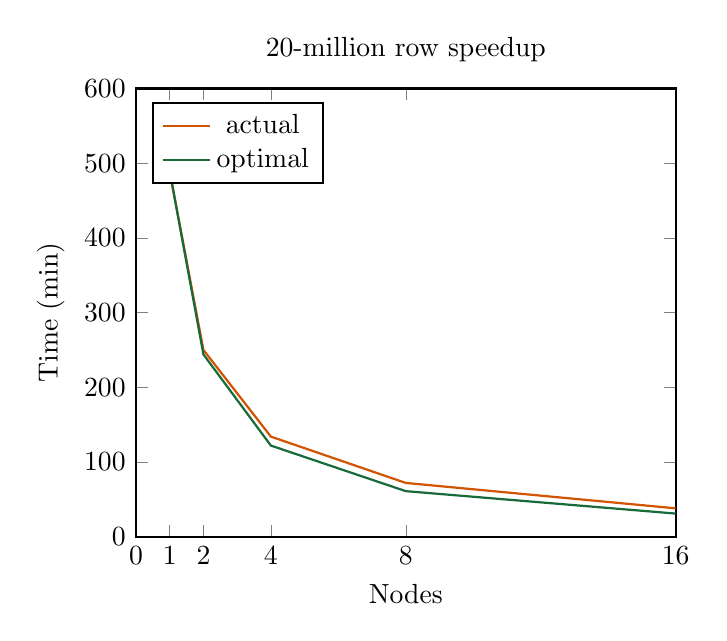
\begin{tikzpicture}
\begin{axis}[
    title={20-million row speedup},
    xlabel={Nodes},
    ylabel={Time (min)},
    xmin=0, xmax=16,
    ymin=0, ymax=600,
    xtick={0, 1,2,4,8,16},
    ytick={0, 100, 200, 300, 400, 500, 600},
    legend pos=north west,
    grid style=dashed,
    style=thick
]

\addplot[color=orange,mark=round]
coordinates {(1,489)(2,250)(4,134)(8,72)(16,38)};

\addplot[color=darkGreen,mark=round]
coordinates {(1,489)(2,244)(4,122)(8,61)(16,31)};

\legend{actual, optimal}
\end{axis}
\end{tikzpicture}


% usage: \includeFig{label}{file}{caption}

% ############################################################################
\section{Conclusions} \label{conclusion}
% ############################################################################

You generally cover three things in the Conclusions section.
\begin{enumerate}
\item Conclusions
\item Summary of Contributions
\item Future Research
\end{enumerate}

Conclusions are not a rambling summary of the thesis: they are short, concise statements of the inferences that you have made because of your work. All conclusions should be directly related to the research question.

The Summary of Contributions will be much sought and carefully read by the readers. Here you list the contributions of new knowledge that your paper makes. Of course, the paper itself must substantiate any claims made here. There is often some overlap with the Conclusions, but that’s okay.

The Future Research should indicate interesting new problems arising from your work. No paper ever solves everything. In fact, the best research papers lead to new research questions for other researchers to work on.


% ############################################################################
% Bibliography
% ############################################################################
\bibliographystyle{plain}
\bibliography{my-bibliography}     %loads my-bibliography.bib

% ============================================================================
\end{document}
% ============================================================================
